\section{Resource Management}

    \subsection{Time Breakdown}
    We have 8 members, each with 200 hours. This means that we have around 1600 hours of total work time. We have allocated around 55 hours each for meetings, workshops and demo time. This makes a total of 440 hours for the group. This leave approximately 1160 hours for working on system. We have broken this time down as follows:
     \subsubsection{Robot}
    \begin{itemize}
        \setlength{\itemindent}{.2in}
        \item Framework : 100
        \item Hatch : 50
        \item Weighing chamber : 50
        \item Selection System : 40
        \item Food bowls : 100
        \item Bluetooth Sensors : 60
        \item Camera : 30
        \item Robot testing: 50
    \end{itemize}
     \subsubsection{Server}
    \begin{itemize}
        \setlength{\itemindent}{.2in}
        \item User Authentication : 10
        \item Send and receive messages from robot and app : 20
        \item Scheduler : 20
        \item Process video : 30
        \item Live stream : 50
        \item Server testing: 40
    \end{itemize}
     \subsubsection{Apps}
    \begin{itemize}
        \setlength{\itemindent}{.2in}
        \item Home page : 20
        \item Sign/login in : 20
        \item Scheduler : 20
        \item Pet analytics : 25
        \item Video : 25
        \item App testing : 50
    \end{itemize}

     \subsubsection{Reports}
    \begin{itemize}
        \setlength{\itemindent}{.2in}
        \item Project Plan : 30
        \item User guide : 40
        \item Technical Report :40
        \item Individual Process Report : 30
    \end{itemize}



     \subsubsection{Demo prep}
    
    \begin{itemize}
        \setlength{\itemindent}{.2in}
        \item Demo 1 : 5
        \item Demo 2 : 5
        \item Demo 3 : 5
        \item Demo 4 : 5
        \item Showcase Demo: 8
    \end{itemize} 
    
    Total time = 968 hours \\
As this is just a rough estimate of how long each task will take, we have left around a further 200 hours as ‘run over’ time should we encounter any problems. 


    \subsection{Technical Subgoals}
    
    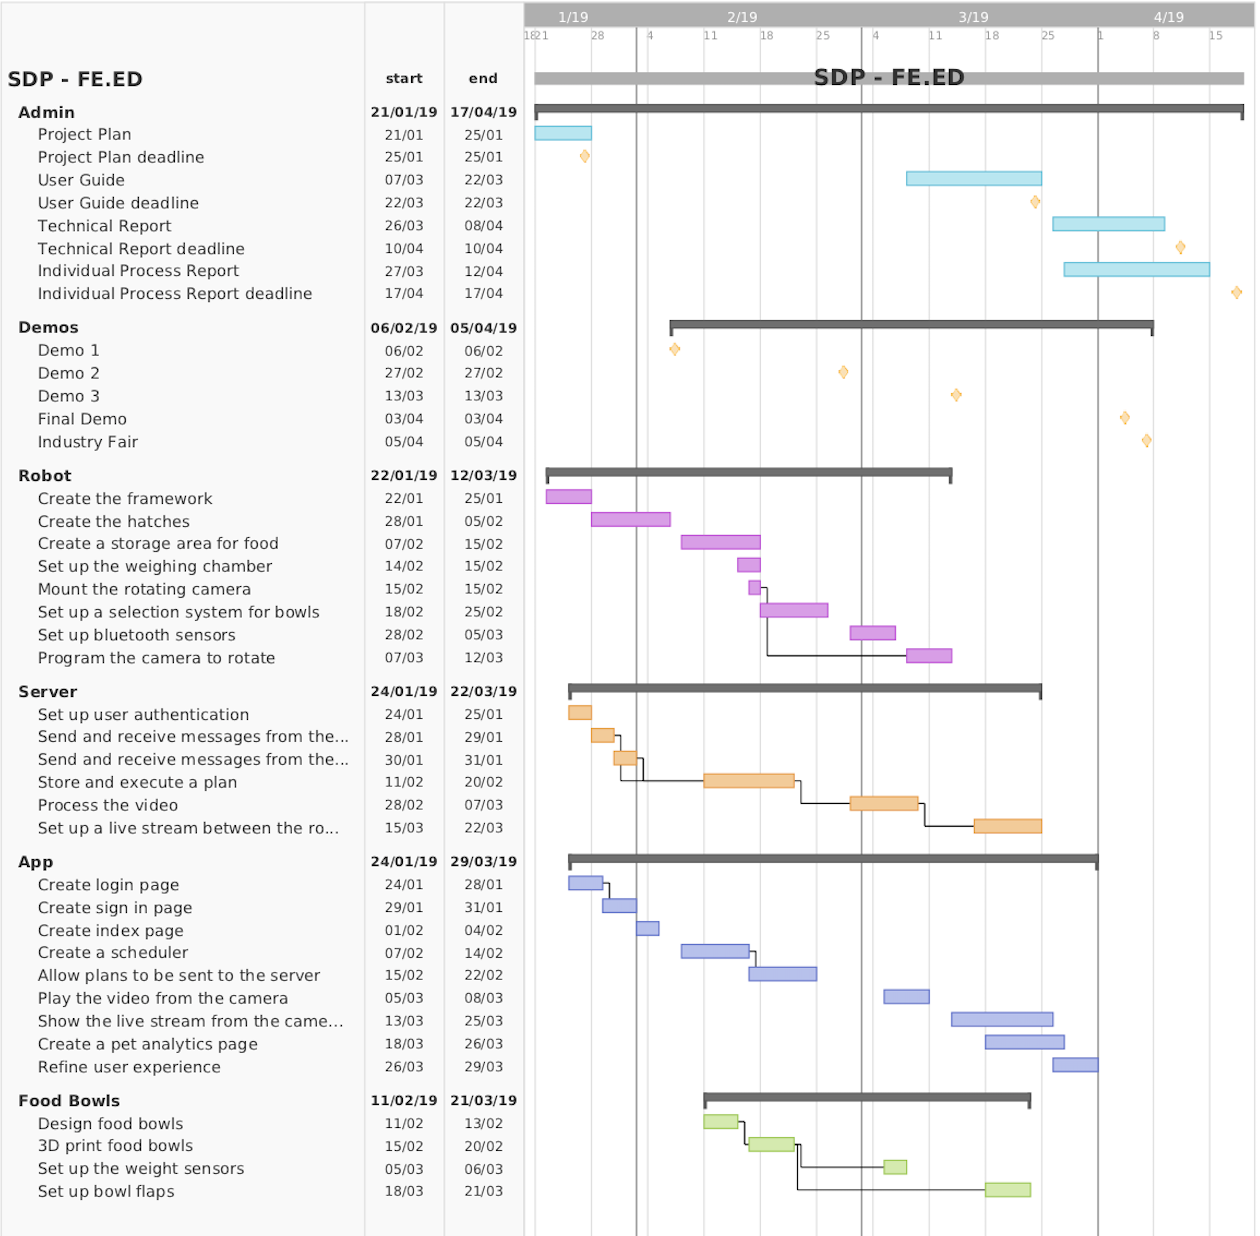
\includegraphics[width=\textwidth]{latex_gantt_chart.png}
    
    \subsection{Skills and Equipment}
    So far, we have identified that we have the following skills which we believe will be important for the project.
    \begin{itemize}
        \setlength{\itemindent}{.2in}
        \item Experience using Spring framework
        \item Experience in web development
        \item Experience with Python
        \item Experience with project management
        \item Experience with version control
        \item Experience with \LaTeX
    \end{itemize}
    For completing the project, we anticipate that we will the need the following equipment. However, as we have not yet started constructing the robot, our required equipment may change over the course of the project. Currently, the main equipment that we have planned to use is as follows:
    \begin{itemize}
        \setlength{\itemindent}{.2in}
        \item 3D printer to print the smart bowls
        \item Bluetooth sensors and chips
        \item Force sensors
        \item Mountable camera
    
    \end{itemize}
We anticipate that we will need to spend a reasonable amount of our funds on these. While we do not have an exact figure, we are aiming to keep a significant amount to use for any other significant purchases that we might need. \par

Similar to the equipment, the skills that we need for the project may change. So far, we have identified the following skills that we need to develop on:
    \begin{itemize}
        \setlength{\itemindent}{.2in}
        \item Design in CAD for 3D printing
        \item Using the React.js framework
        \item Robotics Design
        \item Passing messages to and from a server
        \item Processing video to and from a server
    \end{itemize}

    \subsection{Risk Management}
    

\begin{tabular}{ ||p{3cm}|p{3cm}|c|p{4cm}|p{4cm}|| } 
 \hline \hline
 \textbf{Risk} & \textbf{Impact} & \textbf{Likelihood} & \textbf{Actions to minimise} & \textbf{Contingency Plan} \\ 
 \hline \hline
The robot is dropped when someone is holding it & 
 The robot breaks or is damaged significantly & 
 25\% & 
The robot will only be picked up by one person when above a table, this minimises the distance it has to fall
When carrying the robot from room to room, we will aim to have 2 people holding the robot at all times.
Don’t run when carrying the robot
 & 
 We will assess the damage deal to the robot
If something is broken then we will keep all the pieces together
We will then rebuild the robot, ensuring that it still functions properly
 \\ 
 \hline
 
 
The robot doesn’t function as intended during a demo & 
The demo goes badly & 
 20\% & 
Test the robot before the demo to ensure that it is working
Implement a freeze on any new updates on the robot in the 12 hours prior to the demo
 & 
Establish what went wrong
Try and fix the problem
Explain to the experts what went wrong
 \\ 
 \hline
 
 The weight sensors in the weighing chamber don’t work&
 The robot can’t dispense an accurate volume of food&
 15\%&
 
As the robot is a prototype, we won’t use overly heavy weights
We will aim to predetermine how much weight the sensors can handle in advance
&
 The hatch can open on a timed system. Using this, we can estimate the weight of food dispensed \\ \hline
 
  The hatch is not structurally sound enough to handle the weight of the food&
  The hatch will open unexpectedly.This means food will be dispensed at the wrong time&
  20\%&
  
As the robot is a prototype, we won’t use overly heavy weights.We will aim to predetermine how much weight the hatch can handle in advance &
  Reinforce the hatch.
Think about a different way to implement the hatch
 \\ \hline
  
   A key milestone is not met by the deadline&
   We are unable to start working on the next part of the system&
   35\%&
   We have tried to be realistic when setting milestones. We have budgeted additional time for running over on tasks
&
   Allocate extra resources if necessary.
Re-evaluate how long the task will take to complete
Revise our plan and explain to the experts accordingly
 \\ \hline
   
    Not balancing SDP workload with other courses and personal life&
    
People’s other academic results may suffer.Will increase stress and make burn out more likely
&
    35\%&
   Encourage people to take breaks from SDP to focus on other things.
We’ve aimed to set reasonable goals that are achievable whilst still maintaining a work-life balance
 &
    Encourage the person to take a break from SDP. Stress in a meeting that it’s important to have a balance
 \\ \hline
    
     
 \hline \hline
\end{tabular}


